\documentclass{school-22.101-notes}
\date{November 30, 2011}

\begin{document}
\maketitle

\topic{Angular Distribution of Elastically Scattered Neutrons }
In CMCS the energy differential cross-section $\sigma_s(E)$ and the angular differential cross section $\sigma_s(\theta_C)$ are constant,
\eqn{\frac{\derivative\sigma_s}{\derivative\Omega_C} = \sigma_s (\theta_C) = \frac{\sigma_s(E)}{4 \pi}  \label{sigma-thetaC}}
This is not the case, however, in Lab CS:
\begin{align}
\sigma_s (\Omega) \dOmega &= \sigma_s (\Omega_C) \dOmega_C \\
\sigma_s (\theta) \sin \theta \dtheta &= \sigma_s (\theta_C) \sin \theta_C \cos \theta_C \\
\sigma_s (\theta) \derivative(\cos \theta_C) &= \sigma_s (\theta_C) \derivative(\cos \theta) \\
\sigma_s (\theta) &= \sigma_s (\theta_C) \frac{\derivative(\cos \theta_C)}{\derivative(\cos \theta)}
\end{align}
Apply Eq.~\ref{theta-to-thetaC} and Eq.~\ref{sigma-thetaC}, we find the cross section in the Lab CS:
\begin{align}
\sigma_s (\theta) &= \frac{\sigma_s (E)}{4 \pi} \frac{(\gamma^2 + 2 \gamma \cos \theta_C + 1)^{3/2}}{1 + \gamma \cos \theta_C}, \fsp \gamma = \frac{1}{A}  \\
\overline{\cos \theta} &= \frac{\int \dOmega \cos \theta \sigma(\theta)}{\int \sigma_s (\theta) \dOmega} \approx \frac{2}{3A} > 0 \label{avg-costheta}
\end{align}
Eq.~\ref{avg-costheta} tells us: although the scattering is isotropic in CMCS, in Lab CS it is biased to be forward scattering \footnote{having a positive average $\cos \theta$ suggests that scattering is biased to be in the range of $0 < \theta < \pi$.}. This he forward scattering approach isotropic as $A$ increase. This point is demonstrated in Figure~\ref{P-vs-u}.
\begin{figure}
    \centering
    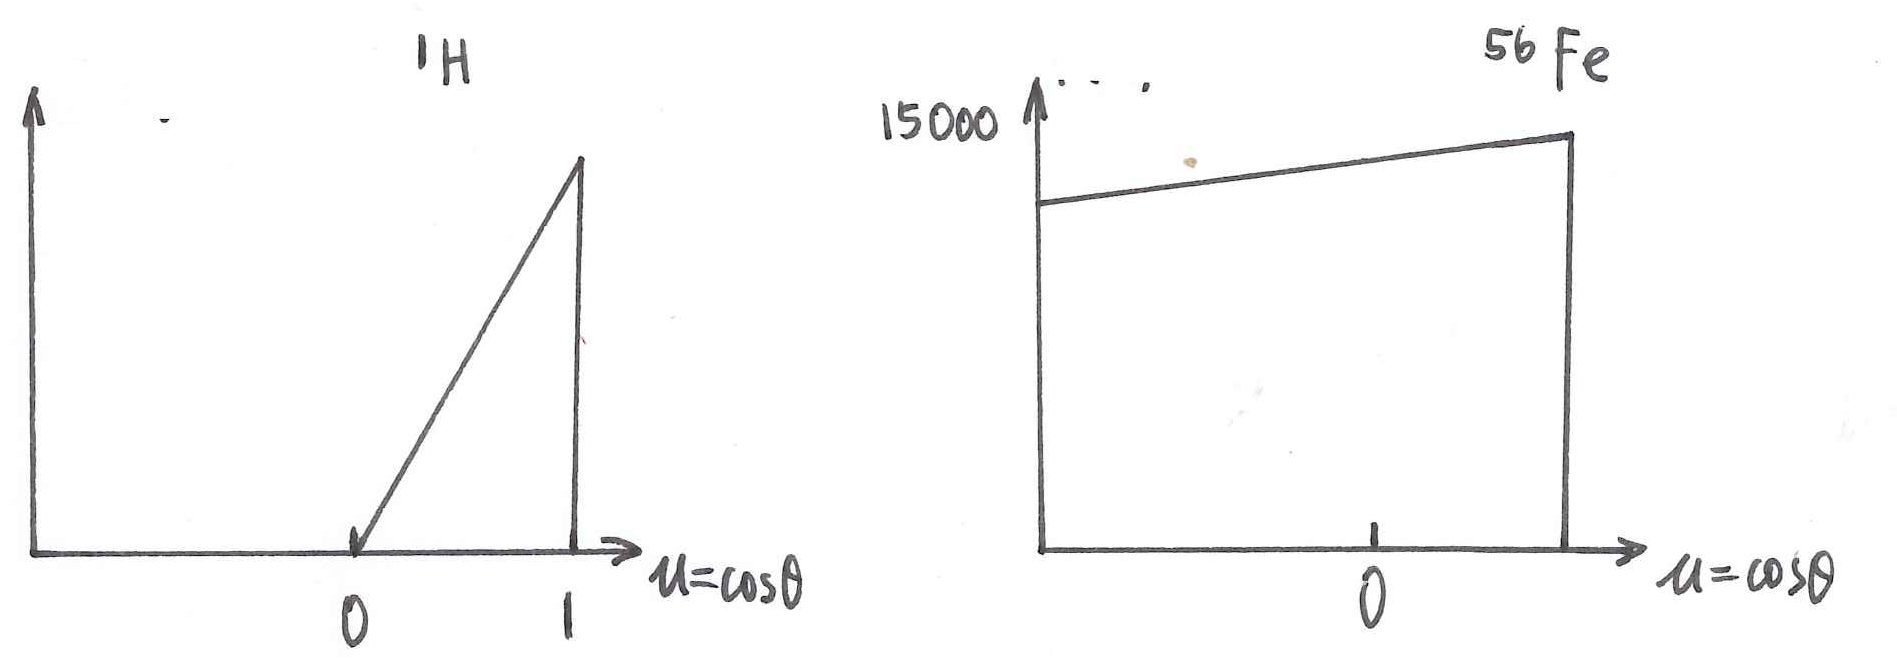
\includegraphics[width=4in]{images/ni/P-vs-u.png}
    \caption{Angular Distribution Depend on A in Lab CS\label{P-vs-u}}
\end{figure}

\topic{Revisit Assumptions}
\begin{enumerate}
\item Elastic Scattering Assumption: this assumption is valid when $E_n$ is small that it does not provide enough energy to excite the compound nucleus, hence the scattering from ground state of $\nu$, no energy lost for excitation. 

If $E_n > 0.05 \sim 0.1$ MeV for heavy nuclei, $E_n > 0.1 \sim 2$ MeV for medium nuclei, it would excite the first nuclear energy level above the ground state, and inelastic scattering becomes energetically possible. Elastic scattering cross section tend to be larger than inelastic scattering cross section: $\sigma (n,n) = 5\sim20$ barns, $\sigma(n,n^{\prime}) \sim 1$ barn.

\item Target at rest: this assumption is valid when neutron energy is large compared to the KE of the target nucleus ($k_B T$): $E_n \gg k_B T$. Typically, $E_n > 0.1$ eV is enough for making this assumption. 

When $E_n \approx k_B T$, neutron energy is around the same level as the thermal motion of the target, and neutron can gain energy from the vibration of the target nucleus as in Figure~\ref{lower-neutron-energy}. 
\begin{figure}
    \centering
    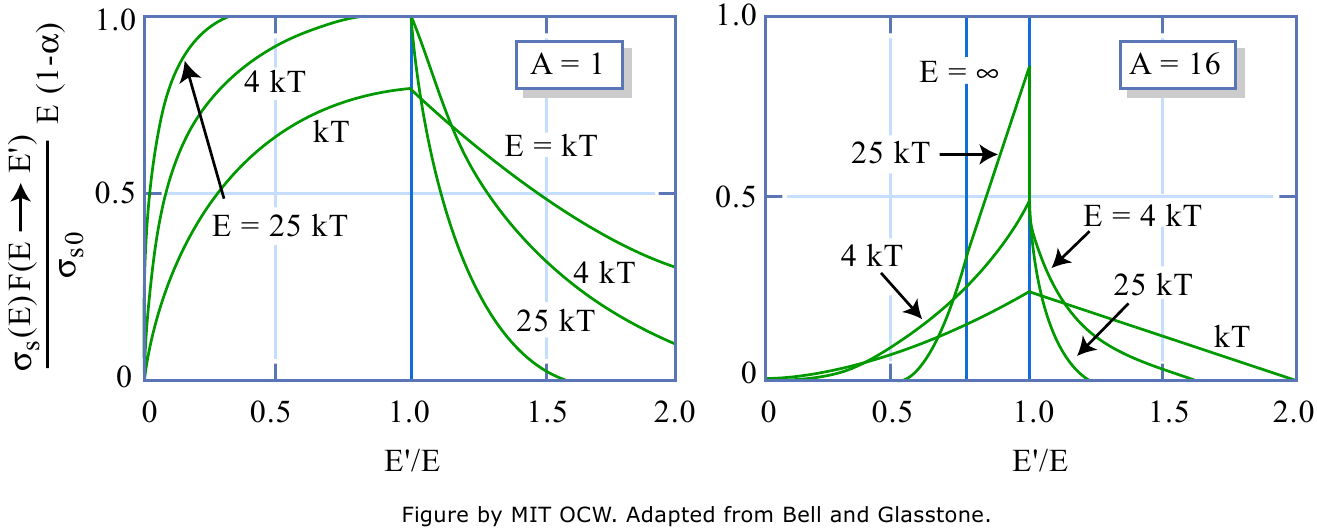
\includegraphics[width=4in]{images/ni/lower-neutron-energy.png}
    \caption{Energy Distribution of Scattering Cross Section, $E_n < k_B T$\label{lower-neutron-energy}}
\end{figure}

\item Isotropic scattering in CMCS: this assumption is valid when $E \ll 10 $keV, $l=0$, S-wave. 

However, if $E > 10$ keV, higher angular momentum (p-wave and above) would be significant, 
\begin{align}
\frac{\derivative\sigma_s}{\dtheta} &= |f(\theta)|^2 = \Sum_l f_l P_l(\cos \theta)  = \underbrace{f_0}_{\mathrm{S-wave}} + \underbrace{f_1 \cos \theta}_{\mathrm{P-wave}} + \cdots \\
\sigma_s (\theta_C) &= \frac{\sigma (E)}{4 \pi} ( 1 + a \cos \theta_C) \\
P(E \to E^{\prime}) \dE^{\prime} &= P(\theta_C) \dtheta_C = P(\cos \theta_C) \derivative (\cos \theta_C) \\
P(\Omega_C) &= \frac{1 + a \cos \theta_C}{4 \pi}, \fsp \fsp P(\theta_C) = \int P(\Omega_C) \dphi \\
P(E^{\prime}) &= \int_0^{2\pi} P(\Omega_C) \dphi \sin \theta_C \frac{\dtheta_C}{\dE^{\prime}} \\
&= \frac{1}{2} (1 + a \cos \theta_C) \sin \theta_C \underbrace{\frac{\dtheta_C}{\dE^{\prime}}}_{- \frac{2}{E(1-\alpha) \sin \theta_C}} \\
&= (1 + a \cos \theta_C) \frac{1}{E(1-\alpha)} \\
&= \frac{a}{\mbox{constant}} + \frac{2 a E^{\prime}}{(1-\alpha)^2 E^2}
\end{align}
See Figure~\ref{p-wave-approx}.
\begin{figure}
    \centering
    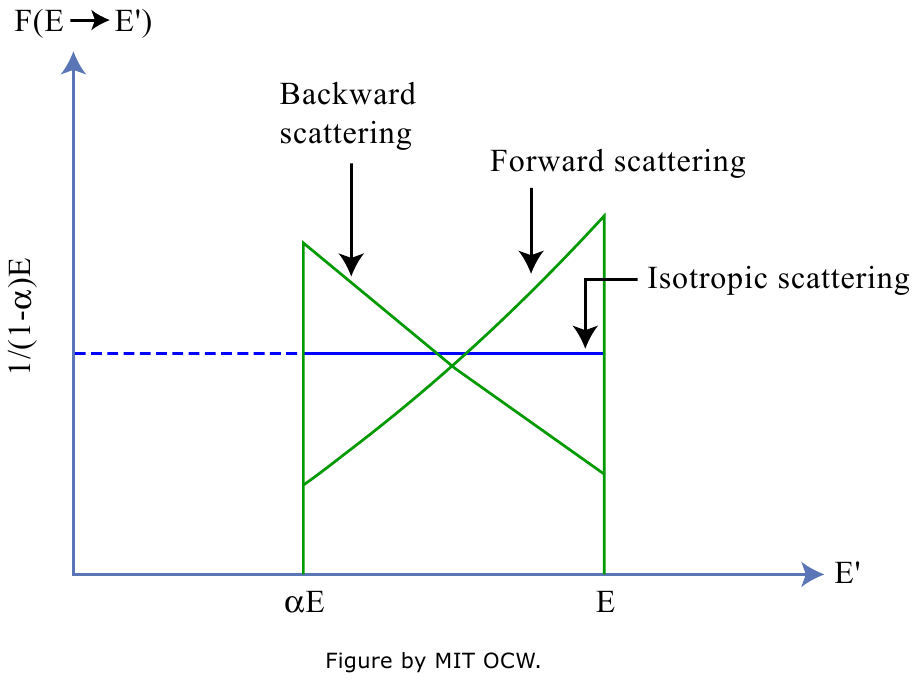
\includegraphics[width=3in]{images/ni/p-wave-approx.png}
    \caption{Energy Distribution of Scattering Cross Section, $E_n > 10$ keV\label{p-wave-approx}}
\end{figure}
\end{enumerate}




\end{document}
